\section{Calibration en énergie des jets dans CMS}\label{chapter-JERC-section-CMS}
% JERC_RunI = 61 : Jet energy scale and resolution in the CMS experiment in \proton\proton\ collisions at \SI{8}{\TeV}
% CMS-DP-2018-028 = 62 : Jet energy scale and resolution performance with \SI{13}{\TeV} data collected by CMS in 2016
% JERC_2011 = 63 : Determination of jet energy calibration and transverse momentum resolution in CMS
Les jets sont des objets composites, complexes, qu'il est nécessaire de calibrer comme tout autre objet reconstruit.
La précision apportée à la mesure des jets est capitale dans de nombreuses analyses, où il s'agit d'une source majeure d'incertitude systématique.
Les avancées réalisées récemment sur la calibration des jets ont ainsi permis d'améliorer la précision sur la mesure de la section efficace inclusive de production de jets et de la masse du quark~\quarkt~\cite{JERC_RunI}.
\par À partir des jets reconstruits par les méthodes décrites précédemment, un procédé de \emph{correction de l'énergie des jets} (JEC\footnote{\emph{Jet Energy Correction}}) est réalisé.
Il permet de corriger l'échelle en énergie des jets (JES\footnote{\emph{Jet Energy Scale}}) ainsi que la résolution sur cette énergie (JER\footnote{\emph{Jet Energy Resolution}}).
La collaboration CMS utilise une approche factorisée dans laquelle plusieurs étapes corrigent un effet en particulier et dépendent des étapes précédentes~\cite{JERC_RunI}.
La figure~\ref{fig-CMS-JME-13-004_Figure_002-TeX} résume ces étapes, décrites plus en détails dans les sections qui suivent.
\begin{figure}[h]
\centering
\includegraphics[width=\textwidth]{\PhDthesisdir/tex/slides/JERC/CMS-JME-13-004_Figure_002-FR-TeX.tex}
\caption{Étapes successives de la JEC pour les données et les simulations~\cite{JERC_RunI}. Les corrections des étapes marquées \og MC \fg{} sont obtenues par l'étude de simulations, celles marquées \og RC \fg{} par une méthode de cône aléatoire (\emph{Random Cone}). Les types d'événements utilisés dans les corrections résiduelles sont également indiqués.}
\label{fig-CMS-JME-13-004_Figure_002-TeX}
\end{figure}
\par Distinguons trois stades ou \og niveaux \fg{} de connaissance sur les particules.
\begin{itemize}
\item Le niveau \emph{particule}, noté \ptcl, ou niveau \og vrai \fg{}, se réfère aux objets et variables après hadronisation mais avant interaction avec le détecteur. Il s'agit donc des grandeurs recherchées, uniquement accessibles dans les événements simulés.
\item Le niveau \emph{reconstruit}, noté \reco, correspond aux objets et variables après interaction avec le détecteur et reconstruction par l'algorithme de \PF.
\item Le niveau \emph{corrigé} ou calibré, noté \cali, correspond aux objets et variables corrigés, \ie\ ceux du niveau \reco\ auxquels ont été appliquées les corrections.
\end{itemize}
Définissons également une variable importante pour ce chapitre, la réponse d'un jet,
\begin{equation}
R = \frac{\pT}{\pT_\ptcl}
\mend
\end{equation}
La réponse peut être définie à différents niveaux, et par définition $R_\ptcl=1$.
Si la JEC est correcte, alors les variables corrigées doivent correspondre aux variables au niveau particule, \ie\ $R_\cali=1$.
Sur la figure~\ref{fig-JERC_RunI-1} sont représentées les réponses de jets d'événements QCD simulés à différentes étapes de la JEC. Après avoir appliqué toutes les corrections, ce qui correspond à la figure~\ref{subfig-JERC_RunI-1_3}, la réponse est sensiblement égal à 1, ce qui montre que la JEC est correcte.
\begin{figure}[h]
\centering
\subcaptionbox{Avant toute correction ($R_\reco$).\label{subfig-JERC_RunI-1_1}}[.31\textwidth]
{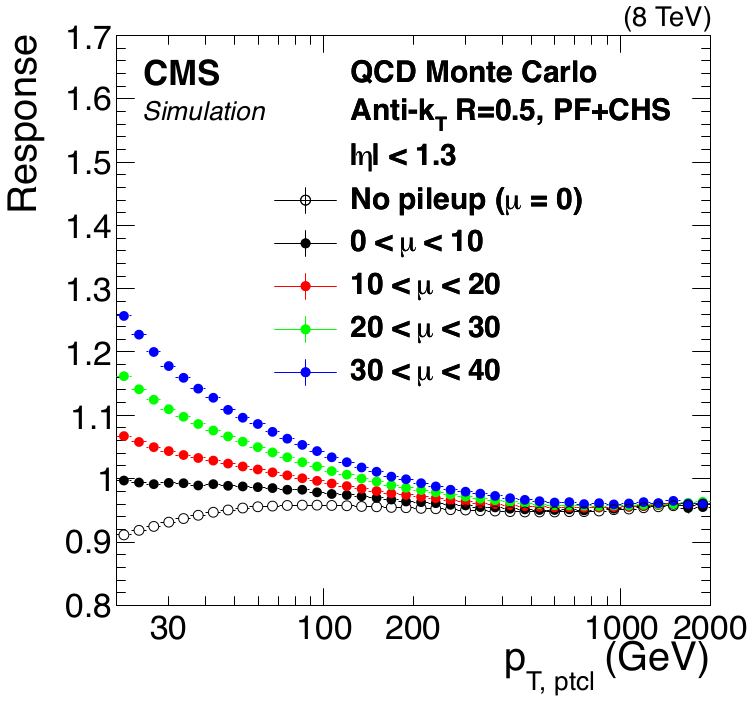
\includegraphics[width=.31\textwidth]{\PhDthesisdir/contents/chapter-JERC/calibration_des_jets/img_from_JERC_RunI/response_evolution_1.png}}
\hfill
\subcaptionbox{Après correction de l'empilement.\label{subfig-JERC_RunI-1_2}}[.31\textwidth]
{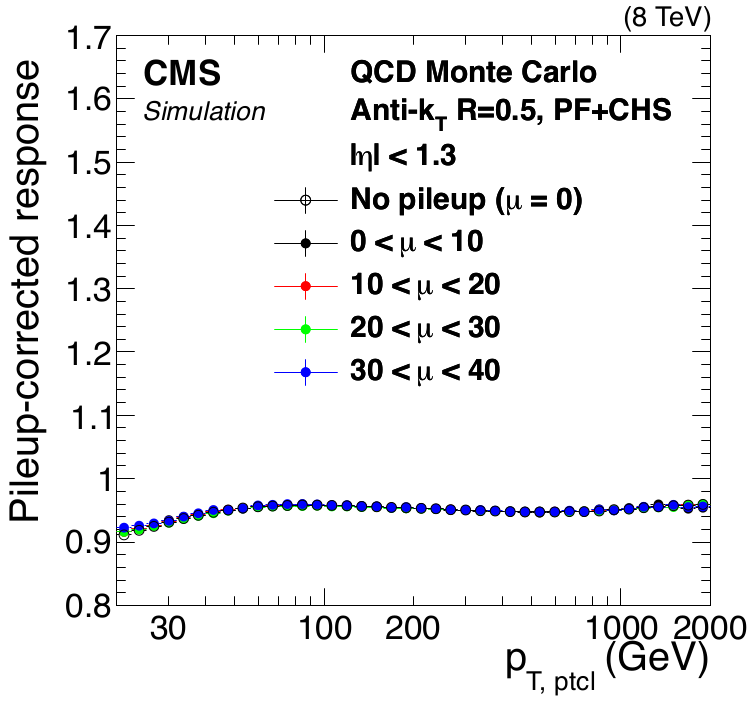
\includegraphics[width=.31\textwidth]{\PhDthesisdir/contents/chapter-JERC/calibration_des_jets/img_from_JERC_RunI/response_evolution_2.png}}
\hfill
\subcaptionbox{Après toutes les corrections ($R_\cali$).\label{subfig-JERC_RunI-1_3}}[.31\textwidth]
{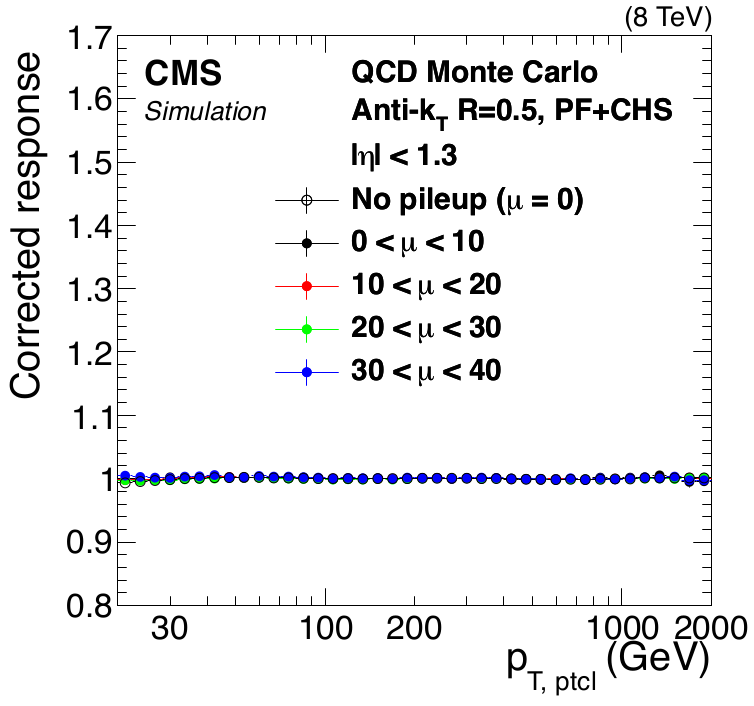
\includegraphics[width=.31\textwidth]{\PhDthesisdir/contents/chapter-JERC/calibration_des_jets/img_from_JERC_RunI/response_evolution_3.png}}
\caption{Valeur moyenne de la réponse de jets d'événements QCD simulés en fonction de $\pT_\ptcl$ à différentes étapes de la JEC~\cite{JERC_RunI} et pour différentes valeurs d'interactions d'empilement $\mu$.}
\label{fig-JERC_RunI-1}
\end{figure}
\par Les jets au niveau particule sont construits en appliquant la procédure de recombinaison à toutes les particules de durée de vie $\tau$ telle que $c\tau>\SI{1}{\centi\meter}$ à l'exception des neutrinos~\cite{JERC_RunI}.
Les hadrons contenant des quarks~\quarkc\ ou~\quarkb\ ne rentrent pas dans cette catégorie et ce sont donc leurs produits de désintégration qui sont pris en compte pour la recombinaison.
Exclure les neutrinos de la recombinaison au niveau particule est une convention adoptée par la collaboration CMS, mais pas de manière universelle en physique des particules.
Les neutrinos sont en fait généralement inclus au niveau particule.
La réponse des jets étant mesurée dans des événements contenant peu de neutrinos, comme cela est discuté dans la section~\ref{chapter-JERC-section-pheno-GJets}, ce choix n'apporte pratiquement aucune différence à la JEC.
L'intérêt de cette convention est de pouvoir définir la réponse des jets d'une manière qui soit accessible expérimentalement et qui réduit significativement les différences de réponse entre jets lourds et jets légers ou de gluons, à cause des neutrinos produits dans les désintégration des quarks lourds.
\subsection{Correction de l'empilement}\label{chapter-JERC-section-CMS-subsec-PU}
Des contributions additionnelles à l'énergie et à l'impulsion des jets peuvent apparaître du fait de l'empilement\footnote{Le phénomène d'empilement est décrit dans la section~\ifref{chapter-LHC-section-LHC-subsec-PU}{\ref{chapter-LHC-section-LHC-subsec-PU}}{1.4} du chapitre\ifref{chapter-LHC}{~\ref{chapter-LHC}}{ \og Dispositif expérimental \fg}.}.
La correction de l'empilement a pour but de soustraire ces contributions et est appliquée dans les données et les événements simulés.
Elle permet d'améliorer la résolution du détecteur et d'obtenir une JES plus précise.
\par L'empilement asynchrone est réduit par l'analyse temporelle des signaux des calorimètres,
l'empilement synchrone par la méthode de soustraction des hadrons chargés (CHS, \emph{Charged Hadron Subtraction}), décrite ci-après.
\par Pour chacun des vertex primaires de l'événement, la somme des impulsions transverses au carré des traces associées au vertex est calculée.
Le vertex primaire principal est choisi comme étant le vertex présentant la plus grande valeur de cette somme.
Les autres vertex primaires sont considérés comme des vertex d'empilement.
Toutes les traces associées aux vertex d'empilement sont retirées de l'événement.
La reconstruction des jets est alors réalisée à partir de l'événement \og nettoyé \fg.
La procédure CHS permet ainsi de supprimer environ \SI{50}{\%} de l'empilement synchrone, uniquement à l'aide du trajectographe.
La correction de l'empilement peut être calculée avec et sans utilisation de la CHS; la JES est peu modifiée par ce choix. Cependant, l'utilisation de la CHS permet d'améliorer la résolution en \pT\ des jets.
L'efficacité de reconstruction des vertex d'empilement étant de \SI{30}{\%}, des traces de hadrons chargés non associées à un vertex subsistent.
De plus, cette méthode ne permet pas de corriger l'empilement des particules neutres.
\par La correction de l'empilement résiduel, principalement due aux particules neutres, aux traces non associées à un vertex et à l'empilement asynchrone qui n'a pas pu être corrigé totalement, est déterminée à l'aide de la méthode de l'aire hybride (\emph{hybrid jet area}).
Il s'agit d'une correction paramétrique, appliquée à chaque jet indépendamment, dépendant de:
\begin{itemize}
\item la densité en énergie dans le plan $(\eta, \phi)$ de l'événement contenant ce jet, $\rho$;
\item l'aire du jet dans le plan $(\eta, \phi)$, $A_j$;
\item la pseudo-rapidité du jet, $\eta$;
\item l'impulsion transverse du jet avant application de cette correction et après CHS, $\pT_\reco^\text{CHS}$.
\end{itemize}
La correction $\mathcal{C}_\text{PU}$ à appliquer à un jet s'exprime alors
\begin{equation}
\mathcal{C}_\text{PU}(\pT_\reco^\text{CHS}, \eta, A_j, \rho)
= 1 - \frac{\left[\rho_0(\eta) + \rho\,\beta(\eta)(1+\gamma(\eta)\log\pT_\reco^\text{CHS})\right]A_j}{\pT_\reco^\text{CHS}}
\label{eq-chapter-JERC-section-CMS-subsec-PU-offset_corr_v1}
\end{equation}
où $\rho_0(\eta)$, $\beta(\eta)$ et $\gamma(\eta)$ sont les paramètres de cette correction, dépendants de $\eta$.
Ils sont déterminés à partir de la contribution additionnelle de l'empilement au niveau particule $\pT_\ptcl^\text{add}$, estimée à partir d'événements QCD multijet simulés avec et sans empilement, telle que
\begin{equation}
\average{\pT_\ptcl^\text{add}}(\rho, \eta, \pT_\reco^\text{CHS})
=
\average{\pT_\ptcl^\text{avec PU} - \pT_\ptcl^\text{sans PU}}
\mend[,]
\label{eq-chapter-JERC-section-CMS-subsec-PU-pTaddptcl}
\end{equation}
avec
$\pT_\ptcl^\text{avec PU}$ et $\pT_\ptcl^\text{sans PU}$
les impulsions du jet au niveau particule avec et sans empilement.
La contribution additionnelle de l'empilement au niveau particule est alors paramétrée en fonction de $\rho$, $\eta$, $\pT_\reco^\text{CHS}$ et $A_j$ afin d'obtenir les paramètres $\rho_0(\eta)$, $\beta(\eta)$ et $\gamma(\eta)$ de l'équation~\eqref{eq-chapter-JERC-section-CMS-subsec-PU-offset_corr_v1} qui peut se réécrire
\begin{equation}
\mathcal{C}_\text{PU}(\pT_\reco^\text{CHS}, \eta, A_j, \rho)
= 1 - \frac{\average{\pT_\ptcl^\text{add}}}{\pT_\reco^\text{CHS}}
\mend
\label{eq-chapter-JERC-section-CMS-subsec-PU-offset_corr_v2}
\end{equation}
La figure~\ref{fig-chapter-JERC-section-CMS-subsec-PU-JERC_RunI-Figure_005} montre $\average{\pT_\ptcl^\text{add}}$ en fonction de l'impulsion transverse du jet au niveau particule, avant et après application de la correction de l'empilement.
Les résultats de la figure~\ref{subfig-chapter-JERC-section-CMS-subsec-PU-JERC_RunI-Figure_005b} sont cohérents avec l'absence d'énergie supplémentaire due à l'empilement à $\pm\SI{0.2}{\GeV}$. Dans le cas d'un grand nombre d'interactions d'empilement ($\mu>30$), un léger effet est visible, lié à une dépendance quadratique en $\rho$ de la contribution en énergie de l'empilement qui n'est pas modélisée~\cite{JERC_RunI}.
\begin{figure}[h]
\centering
\subcaptionbox{Avant correction.\label{subfig-chapter-JERC-section-CMS-subsec-PU-JERC_RunI-Figure_005a}}[8.1cm]
{\begin{tikzpicture}
\node[anchor=south west,inner sep=0] at (0,0) {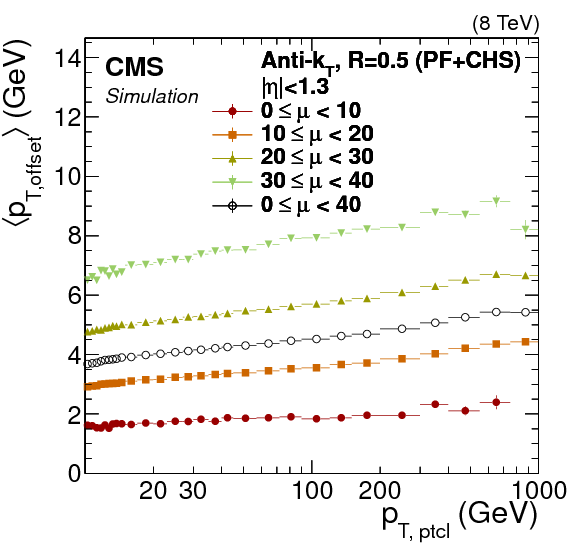
\includegraphics[width=8cm]{\PhDthesisdir/contents/chapter-JERC/calibration_des_jets/img_from_JERC_RunI/Figure_005-a.png}};
\fill [white] (0, 4) rectangle + (.65, 3.5);
\draw (.3, 7.2) node [left, rotate=90] {$\average{\pT_\ptcl^\text{add}}$ (\SI{}{\GeV})};
\fill [white] (5, 0) rectangle + (2.6, .625);
\draw (6.5, .3) node {$\pT_\ptcl$ (\SI{}{\GeV})};
\end{tikzpicture}}
\hfill
\subcaptionbox{Après correction.\label{subfig-chapter-JERC-section-CMS-subsec-PU-JERC_RunI-Figure_005b}}[8.1cm]
{\begin{tikzpicture}
\node[anchor=south west,inner sep=0] at (0,0) {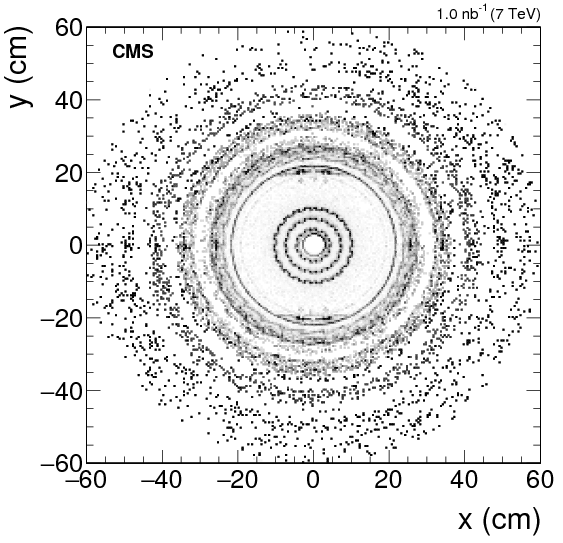
\includegraphics[width=8cm]{\PhDthesisdir/contents/chapter-JERC/calibration_des_jets/img_from_JERC_RunI/Figure_005-b.png}};
\fill [white] (0, 4) rectangle + (.65, 3.5);
\draw (.3, 7.2) node [left, rotate=90] {$\average{\pT_\ptcl^\text{add}}$ (\SI{}{\GeV})};
\fill [white] (5, 0) rectangle + (2.6, .625);
\draw (6.5, .3) node {$\pT_\ptcl$ (\SI{}{\GeV})};
\end{tikzpicture}}
\caption{Contribution additionnelle de l'empilement au niveau particule telle que définie dans l'équation~\eqref{eq-chapter-JERC-section-CMS-subsec-PU-pTaddptcl} pour $\abs{\eta}<\num{1.3}$ en fonction de l'impulsion du jet au niveau particule pour différentes valeurs du nombre d'interaction d'empilement ($\mu$)~\cite{JERC_RunI}.}
\label{fig-chapter-JERC-section-CMS-subsec-PU-JERC_RunI-Figure_005}
\end{figure}
\par La correction ainsi décrite doit être légèrement adaptée pour pouvoir l'appliquer aux données à cause des biais de simulation du détecteur.
Pour cela, un ajustement en fonction de $\eta$ est déterminé à l'aide de la méthode de cône aléatoire (RC, \emph {Random Cone}). La méthode RC reconstruit les jets à l'aide de cônes dont la direction en $(\eta, \phi)$ est choisie de manière aléatoire.
L'étude est réalisée sur des événements dits de \og zéro biais \fg, dans lesquels aucune énergie provenant d'une interaction dure\footnote{\todo{définir?}} n'est présente.
Dans ce cas, la valeur moyenne du \pT\ des jets reconstruits par la méthode RC permet d'estimer la moyenne de la contribution additionnelle de l'empilement, \ie
\begin{equation}
\average{\pT^\text{add}}^\text{RC} = \average{\pT_\text{cône}}
\mend
\end{equation}
Il est alors possible de définir un facteur d'échelle à appliquer aux paramètres $\rho_0$ et $\beta$ de l'équation~\eqref{eq-chapter-JERC-section-CMS-subsec-PU-offset_corr_v1} lorsque cette correction est appliquée aux données. Ce facteur d'échelle s'exprime
\begin{equation}
\frac{\average{\pT^\text{add}}^\text{RC}_\text{données}(\eta, \rho_\text{données})}{\average{\pT^\text{add}}^\text{RC}_\text{simulation}(\eta, \rho_\text{simulation})}
\mend
\end{equation}
La contribution additionnelle de l'empilement est ainsi corrigée dans les simulations et les données.
\subsection{Correction de la réponse du détecteur en $\pT$ et en $\eta$}\label{chapter-JERC-section-CMS-subsec-reponse}
La réponse du détecteur CMS à un jet n'est pas uniforme selon la valeur de \pT\ et $\eta$ du jet.
La réponse au niveau reconstruit de jets simulés $R_\reco$,
déterminée grâce à une simulation du détecteur CMS basée sur \GEANTfour~\cite{geant4},
combinée à \PYTHIA~6.4~\cite{pythia6.4}
avec les réglages Z2*~\cite{Khachatryan:2015pea},
est représentée sur la figure~\ref{fig-simulated_jet_response_RunII} pour les trois années du Run~II du LHC.
Il apparaît, par exemple, qu'un jet de $\pT=\SI{30}{\GeV}$ nécessite une correction allant de \SI{10}{\%} dans la région centrale $\abs{\eta}<\num{0.7}$ à plus de \SI{30}{\%} lorsque $\abs{\eta}\simeq\num{3}$ en 2017 et 2018.
\begin{figure}[h]
\centering
\subcaptionbox{Année 2016.\label{subfig-simulated_jet_response_2016}}[.31\textwidth]
{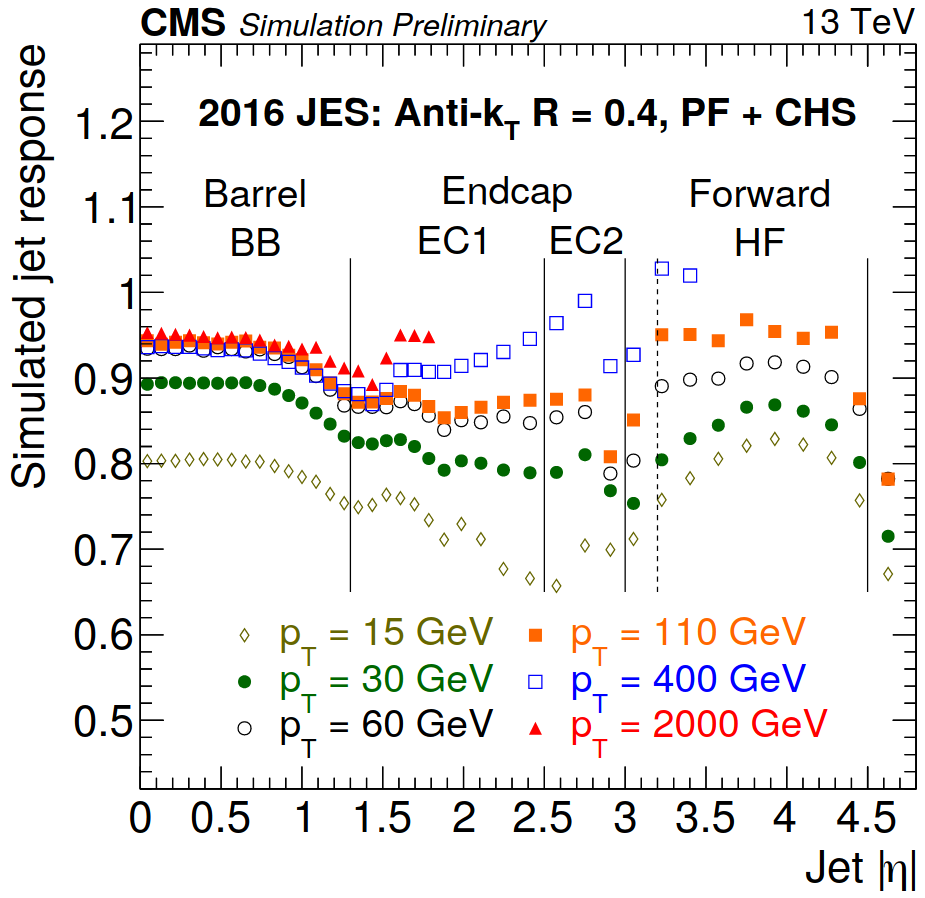
\includegraphics[width=.31\textwidth]{\PhDthesisdir/contents/chapter-JERC/calibration_des_jets/simulated_jet_response_2016_CMS-DP-2018-028.png}}
\hfill
\subcaptionbox{Année 2017.\label{subfig-simulated_jet_response_2017}}[.31\textwidth]
{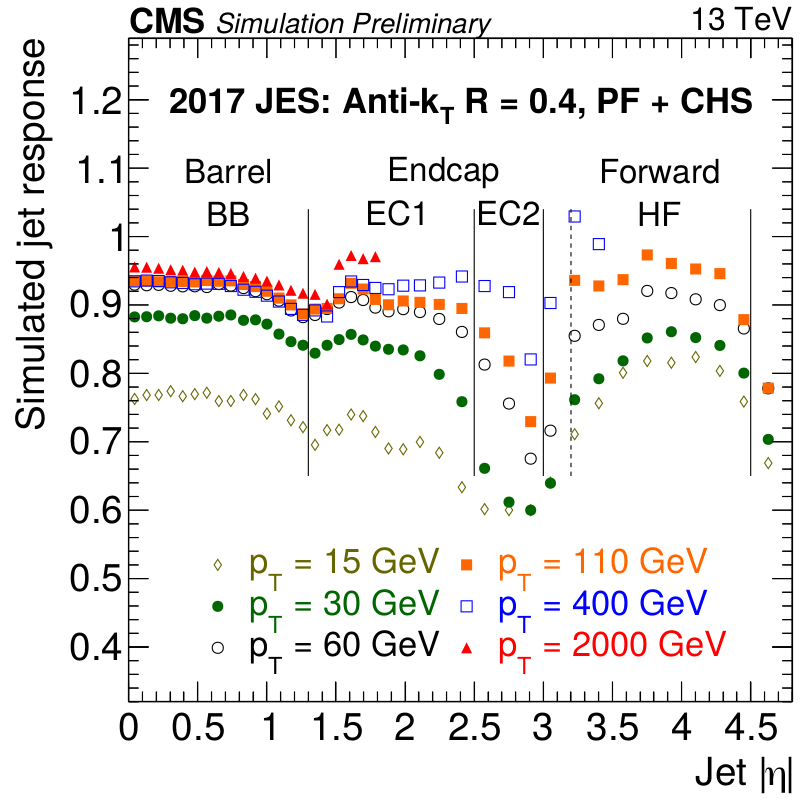
\includegraphics[width=.31\textwidth]{\PhDthesisdir/contents/chapter-JERC/calibration_des_jets/simulated_jet_response_2017.png}}
\hfill
\subcaptionbox{Année 2018.\label{subfig-simulated_jet_response_2018}}[.31\textwidth]
{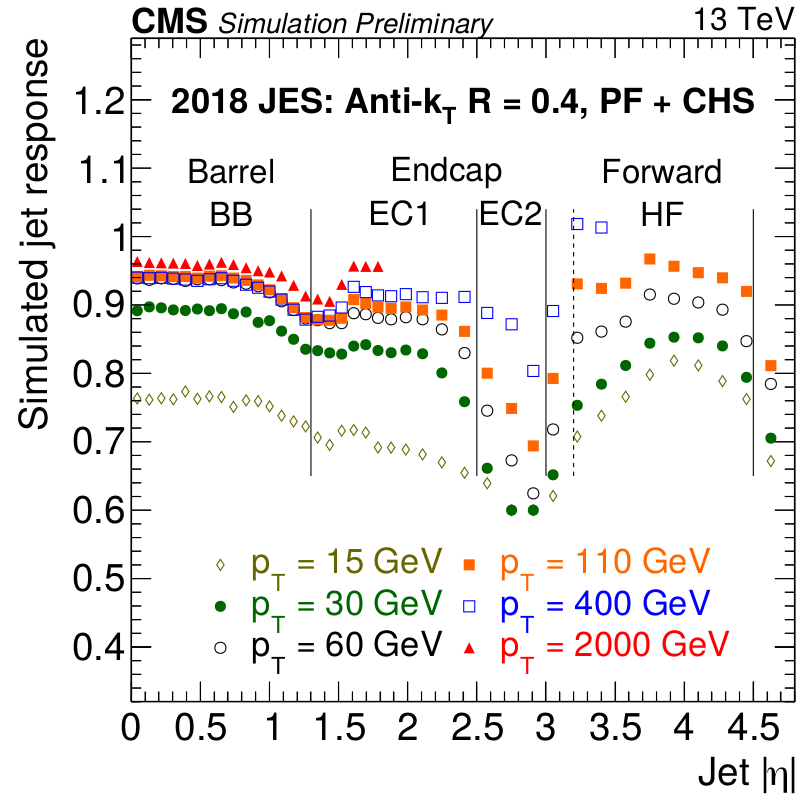
\includegraphics[width=.31\textwidth]{\PhDthesisdir/contents/chapter-JERC/calibration_des_jets/simulated_jet_response_2018.png}}
\caption{Réponse des jets reconstruits en fonction de \pT\ et $\eta$ lors du Run~II. La baisse dans la région $\num{3.0}<\abs{\eta}<\num{3.2}$ (respectivement $\abs{\eta}>\num{4.5}$) est due à la transition le bouchon (\emph{endcap}) et la partie avancée (\emph{forward}) du détecteur (reps. son acceptation). La dégradation au cours du temps du détecteur dans la région \og EC2 \fg{} s'observe par la baisse de la réponse des jets dans cette région de 2016 à 2017.}
\label{fig-simulated_jet_response_RunII}
\end{figure}
\par Afin de corriger la réponse du détecteur en $\pT$ et en $\eta$, la correction $\mathcal{C}_\text{Rép}$ à appliquer s'exprime
\begin{equation}
\mathcal{C}_\text{Rép}(\pT_\reco', \eta) = \frac{\average{\pT_\ptcl}}{\average{\pT_\reco'}} = \frac{1}{\average{R_\reco'}}
\end{equation}
où $\pT_\reco'$ est l'impulsion transverse du jet après correction de l'empilement.
Les moyennes sont réalisées sur les jets appartenant à la même cellule d'une grille en $(\pT_\ptcl, \eta)$ prédéfinie~\cite{JERC_RunI}.
\subsection{Propagation à la MET}\label{chapter-JERC-section-CMS-subsec-MET}

\subsection{Corrections résiduelles}\label{chapter-JERC-section-CMS-subsec-residuals}
une fois le ECAL calibré (test de presque chaque cristal en faisceau), calibration du HCAL.

see end of page 3, beg. p.4

\subsection{Correction de la résolution en énergie}\label{chapter-JERC-section-CMS-subsec-JER}
The jet p T resolution, measured after applying JEC, is extracted in data and simulated events.
It is studied as a function of pileup, jet size R, and jet flavor. The effect of the presence of
neutrinos in the jets is also studied. The typical JER is 15–20% at 30 GeV, about 10% at 100 GeV,
and 5% at 1 TeV at central rapidities.


The jet p T resolutions are determined with both dijet and photon+jet events, as discussed in
Section 8. The reference resolutions obtained from simulation are parameterized as a function
of particle-level jet pTptcl (defined in Section 2) and average number $\mu$ of PU interactions in bins of jet $\eta$.
Corrections for differences between data and MC simulation are applied as
$\eta$-binned scale factors.

\subsection{Incertitudes}\label{chapter-JERC-section-CMS-subsec-unc}
The JES uncertainties, discussed in Section 9, are provided in the form of a limited set of sources
that allow a detailed statistical analysis of uncertainty correlations. The final uncertainties are
below 1\% across much of the phase space covered by these corrections at p T > 10 GeV and
$\abs{\eta} < 5.2$. This sets a new benchmark for jet energy scale at hadron colliders.


\subsection{•}
The optional jet-flavor corrections derived from MC simulation are discussed in Section 7 together with the JEC flavor uncertainty estimates based on comparing PYTHIA 6.4 and HERWIG ++2.3 predictions. These uncertainties are applicable to data vs. simulation comparisons regardless of whether or not the jet-flavor corrections are applied. The flavor corrections and their uncertainties for b-quark jets are checked in data with Z+b events.